\newpage

\colorlet{cluster1}{blue!25}
\colorlet{cluster3}{gray}
\definecolor{cluster3}{rgb}{0.88,1,1}
\begin{table}[h]
    \begin{center}
      \caption{Histograma - Resultado do conjunto chaves em 3 grupos.}
\begin{tabular}{ |>{\centering\arraybackslash}m{4.9cm} | >{\centering\arraybackslash}m{4.9cm} | >{\centering\arraybackslash}m{4.9cm} | } 
	\hline
	\cellcolor{cluster1}
   \grbox{
   \begin{subfigure}[b]{5cm}
   \centering
   
\includegraphics[width=5cm,height=2cm,keepaspectratio,trim=0 0 0 -5]{images/chaves/0.jpeg} 
	\end{subfigure}}{0}
   &
   \cellcolor{cluster1}
    \grbox{
   \begin{subfigure}[b]{5cm}
  \centering
   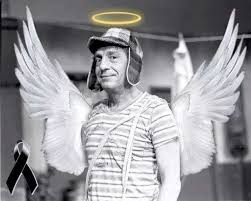
\includegraphics[width=5cm,height=2cm,keepaspectratio,trim=0 0 0 -5]{images/chaves/29.jpeg} 
	\end{subfigure}}{\underline{29}}
   & 
   \cellcolor{cluster1}
    \grbox{
   \begin{subfigure}[b]{5cm}
  \centering
   
\includegraphics[width=5cm,height=2cm,keepaspectratio,trim=0 0 0 -5]{images/chaves/30.jpeg} 
	\end{subfigure}}{30}
 \\ 
 \cellcolor{cluster2}
   \grbox{
   \begin{subfigure}[b]{5cm}
  \centering
   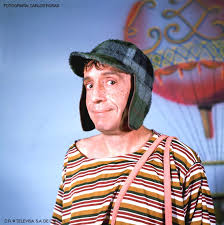
\includegraphics[width=5cm,height=2cm,keepaspectratio,trim=0 0 0 -5]{images/chaves/8.jpeg} 
	\end{subfigure}}{\underline{8}}
   &
   \cellcolor{cluster2}
   \grbox{
   \begin{subfigure}[b]{5cm}
  \centering
   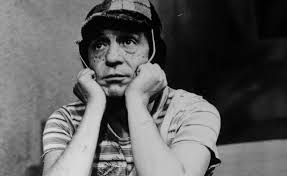
\includegraphics[width=5cm,height=2cm,keepaspectratio,trim=0 0 0 -5]{images/chaves/31.jpeg} 
	\end{subfigure}}{31}
   & 
   \cellcolor{cluster3}
   \grbox{
   \begin{subfigure}[b]{5cm}
  \centering
    
\includegraphics[width=5cm,height=2cm,keepaspectratio,trim=0 0 0 -5]{images/chaves/2.jpeg} 
	\end{subfigure}}{2}
 \\ 
   \cellcolor{cluster3}
   \grbox{
   \begin{subfigure}[b]{5cm}
  \centering
   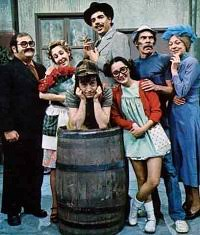
\includegraphics[width=5cm,height=2cm,keepaspectratio,trim=0 0 0 -5]{images/chaves/4.jpeg} 
	\end{subfigure}}{4}
   &
   \cellcolor{cluster3}
   \grbox{
   \begin{subfigure}[b]{5cm}
  \centering
   
\includegraphics[width=5cm,height=2cm,keepaspectratio,trim=0 0 0 -5]{images/chaves/5.jpeg} 
	\end{subfigure}}{5}
   & 
   \cellcolor{cluster3}
   \grbox{
   \begin{subfigure}[b]{5cm}
  \centering
    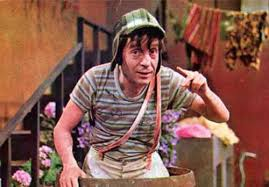
\includegraphics[width=5cm,height=2cm,keepaspectratio,trim=0 0 0 -5]{images/chaves/3.jpeg} 
	\end{subfigure}}{3}
 \\ 
   
   \cellcolor{cluster3}
   \grbox{
   \begin{subfigure}[b]{5cm}
  \centering
   
\includegraphics[width=5cm,height=2cm,keepaspectratio,trim=0 0 0 -5]{images/chaves/6.jpeg} 
	\end{subfigure}}{\underline{6}}
   &
   \cellcolor{cluster3}
   \grbox{
   \begin{subfigure}[b]{5cm}
  \centering
   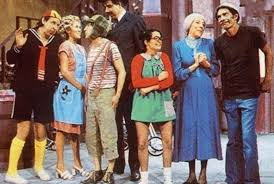
\includegraphics[width=5cm,height=2cm,keepaspectratio,trim=0 0 0 -5]{images/chaves/7.jpeg} 
	\end{subfigure}}{7}
   & 
   \cellcolor{cluster3}
   \grbox{
   \begin{subfigure}[b]{5cm}
  \centering
    
\includegraphics[width=5cm,height=2cm,keepaspectratio,trim=0 0 0 -5]{images/chaves/9.jpeg} 
	\end{subfigure}}{9}
 \\ 
   
   \cellcolor{cluster3}
   \grbox{
   \begin{subfigure}[b]{5cm}
  \centering
   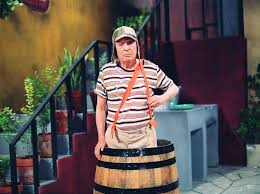
\includegraphics[width=5cm,height=2cm,keepaspectratio,trim=0 0 0 -5]{images/chaves/1.jpeg} 
	\end{subfigure}}{1}
   &
   \cellcolor{cluster3}
   \grbox{
   \begin{subfigure}[b]{5cm}
  \centering
   
\includegraphics[width=5cm,height=2cm,keepaspectratio,trim=0 0 0 -5]{images/chaves/16.jpeg} 
	\end{subfigure}}{16}
   & 
   \cellcolor{cluster3}
   \grbox{
   \begin{subfigure}[b]{5cm}
  \centering
    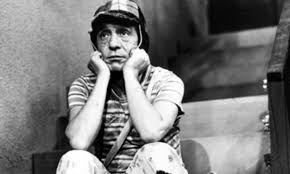
\includegraphics[width=5cm,height=2cm,keepaspectratio,trim=0 0 0 -5]{images/chaves/12.jpeg} 
	\end{subfigure}}{12}
 \\ 
   
   \cellcolor{cluster3}
   \grbox{
   \begin{subfigure}[b]{5cm}
  \centering
   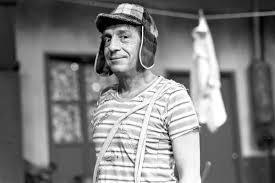
\includegraphics[width=5cm,height=2cm,keepaspectratio,trim=0 0 0 -5]{images/chaves/17.jpeg} 
	\end{subfigure}}{17}
   &
   \cellcolor{cluster3}
   \grbox{
   \begin{subfigure}[b]{5cm}
  \centering
   
\includegraphics[width=5cm,height=2cm,keepaspectratio,trim=0 0 0 -5]{images/chaves/19.jpeg} 
	\end{subfigure}}{19}
   & 
   \cellcolor{cluster3}
   \grbox{
   \begin{subfigure}[b]{5cm}
  \centering
    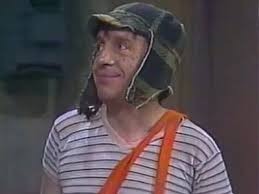
\includegraphics[width=5cm,height=2cm,keepaspectratio,trim=0 0 0 -5]{images/chaves/27.jpeg} 
	\end{subfigure}}{27}
 \\ 
   
   \cellcolor{cluster3}
   \grbox{
   \begin{subfigure}[b]{5cm}
  \centering
   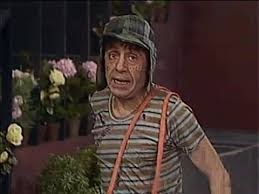
\includegraphics[width=5cm,height=2cm,keepaspectratio,trim=0 0 0 -5]{images/chaves/18.jpeg} 
	\end{subfigure}}{18}
   &
   \cellcolor{cluster3}
   \grbox{
   \begin{subfigure}[b]{5cm}
  \centering
   
\includegraphics[width=5cm,height=2cm,keepaspectratio,trim=0 0 0 -5]{images/chaves/10.jpeg} 
	\end{subfigure}}{10}
   & 
   \cellcolor{cluster3}
   \grbox{
   \begin{subfigure}[b]{5cm}
  \centering
    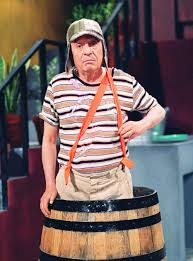
\includegraphics[width=5cm,height=2cm,keepaspectratio,trim=0 0 0 -5]{images/chaves/11.jpeg} 
	\end{subfigure}}{11}
 \\ 
   
   \cellcolor{cluster3}
   \grbox{
   \begin{subfigure}[b]{5cm}
  \centering
   
\includegraphics[width=5cm,height=2cm,keepaspectratio,trim=0 0 0 -5]{images/chaves/13.jpeg} 
	\end{subfigure}}{13}
   &
   \cellcolor{cluster3}
   \grbox{
   \begin{subfigure}[b]{5cm}
  \centering
   
\includegraphics[width=5cm,height=2cm,keepaspectratio,trim=0 0 0 -5]{images/chaves/14.jpeg} 
	\end{subfigure}}{14}
   & 
   \cellcolor{cluster3}
   \grbox{
   \begin{subfigure}[b]{5cm}
  \centering
    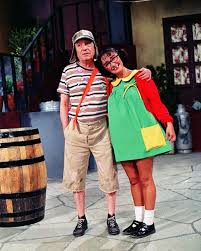
\includegraphics[width=5cm,height=2cm,keepaspectratio,trim=0 0 0 -5]{images/chaves/15.jpeg} 
	\end{subfigure}}{15}
 \\
 
 \cellcolor{cluster3}
 \grbox{
   \begin{subfigure}[b]{5cm}
  \centering
   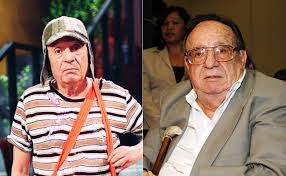
\includegraphics[width=5cm,height=2cm,keepaspectratio,trim=0 0 0 -5]{images/chaves/20.jpeg} 
	\end{subfigure}}{20}
   &
   \cellcolor{cluster3}
   \grbox{
   \begin{subfigure}[b]{5cm}
  \centering
   
\includegraphics[width=5cm,height=2cm,keepaspectratio,trim=0 0 0 -5]{images/chaves/21.jpeg} 
	\end{subfigure}}{21}
   & 
   \cellcolor{cluster3}
   \grbox{
   \begin{subfigure}[b]{5cm}
  \centering
    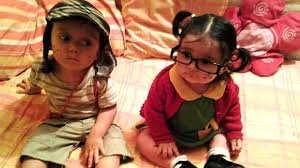
\includegraphics[width=5cm,height=2cm,keepaspectratio,trim=0 0 0 -5]{images/chaves/22.jpeg} 
	\end{subfigure}}{22}
 \\
  \cellcolor{cluster3}
 \grbox{
   \begin{subfigure}[b]{5cm}
  \centering
   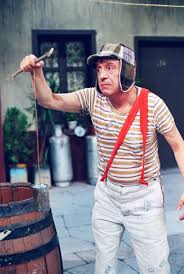
\includegraphics[width=5cm,height=2cm,keepaspectratio,trim=0 0 0 -5]{images/chaves/23.jpeg} 
	\end{subfigure}}{23}
   &
   \cellcolor{cluster3}
   \grbox{
   \begin{subfigure}[b]{5cm}
  \centering
   
\includegraphics[width=5cm,height=2cm,keepaspectratio,trim=0 0 0 -5]{images/chaves/24.jpeg} 
	\end{subfigure}}{24}
   & 
   \cellcolor{cluster3}
   \grbox{
   \begin{subfigure}[b]{5cm}
  \centering
    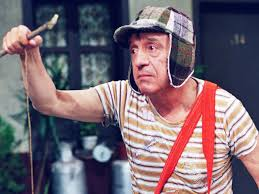
\includegraphics[width=5cm,height=2cm,keepaspectratio,trim=0 0 0 -5]{images/chaves/26.jpeg} 
	\end{subfigure}}{26}
 \\
 \cellcolor{cluster3}
 \grbox{
   \begin{subfigure}[b]{5cm}
  \centering
   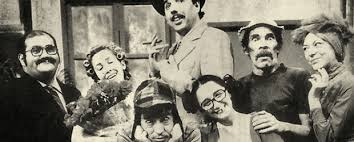
\includegraphics[width=4.2cm,height=2cm,keepaspectratio,trim=0 0 0 -5]{images/chaves/25.jpeg} 
	\end{subfigure}}{25}
   &
   \cellcolor{cluster3}
   \grbox{
   \begin{subfigure}[b]{5cm}
  \centering
   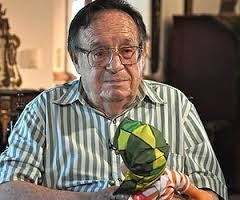
\includegraphics[width=5cm,height=2cm,keepaspectratio,trim=0 0 0 -5]{images/chaves/28.jpeg} 
	\end{subfigure}}{28}
   &
   \cellcolor{cluster3}
   \grbox{
   \begin{subfigure}[b]{5cm}
  \centering
   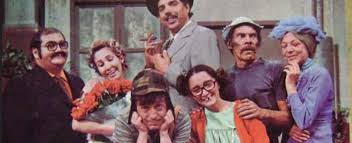
\includegraphics[width=4.2cm,height=2cm,keepaspectratio,trim=0 0 0 -5]{images/chaves/32.jpeg} 
	\end{subfigure}}{32}
  \\
  \hline
\end{tabular}
\label{chavesHistograma}
\legend{\textbf{Fonte:} \citeonline{google2}.}
\end{center}
\end{table}